% Makros zur Kompatibilitaet mit Onlinemodul: 
 \providecommand{\MoIl}[1][]{\mbox{}#1]\mathopen{}} 
 \providecommand{\MoIr}[1][]{#1[\mbox{}} 
 \providecommand{\MIntvlSep}{;} 
 \providecommand{\MElSetSep}{\, ; \, } 
 \begin{MAufgabe}{Lineare Betrags(un)gleichungen}{vr, 2016, MaTeX}
L\"osen Sie die Gleichung
$$
 \MDS 5\left| 3\, x - 1 \right|1=  \left|  - 2\, x - 2 \right| +x + 3
$$  

\ifLsg\MLoesung

Im ersten Schritt k\"onnen die Terme au\ss{}erhalb der Betragszeichen zusammengefasst werden:

\begin{align*} 
 5\left| 3\, x - 1 \right|1=  \left|  - 2\, x - 2 \right| +x + 3\\ 
\Leftrightarrow5\, \left|3\, x - 1\right| - \left|2\, x + 2\right| - x - 2= 0 
 \end{align*}

F\"ur diese Gleichung haben wir 4 F\"alle zu unterscheiden: 
\begin{enumerate}
\item $ \MDS 
\begin{cases} 
 0 \leq 3\, x - 1\\ 
0 \leq  - 2\, x - 2
 \end{cases}
 \mbox{ : keine L\"osung. Diese Bedingung ist nirgendwo erf\"ullt.}$ 
\item $ \MDS 
\begin{cases} 
 0 \leq 3\, x - 1\\ 
 - 2\, x - 2 < 0
 \end{cases}
\Leftrightarrow \frac{1}{3} \leq x\Leftrightarrow x \in [ \frac{1}{3} \, \MIntvlSep \, \infty\MoIr $ 
\item $ \MDS 
\begin{cases} 
 3\, x - 1 < 0\\ 
0 \leq  - 2\, x - 2
 \end{cases}
\Leftrightarrow x \leq -1\Leftrightarrow x \in \MoIl  -\infty \, \MIntvlSep \, -1]$ 
\item $ \MDS 
\begin{cases} 
 3\, x - 1 < 0\\ 
 - 2\, x - 2 < 0
 \end{cases}
\Leftrightarrow -1 < x \wedge x < \frac{1}{3}\Leftrightarrow x \in \MoIl  -1 \, \MIntvlSep \, \frac{1}{3}\MoIr $ 
\end{enumerate} 
Der 1. Fall ist nirgendwo erf\"ullt. Betrachte weiter nur die restlichen F\"alle.
 
 Fallunterscheidung: 

 \begin{enumerate} 
 \item Sei $ \MDS x\in[ \frac{1}{3} \, \MIntvlSep \, \infty\MoIr $. 
 In diesem Fall gilt: 
  $ \MDS \left| 3\, x - 1\right|=3\, x - 1$ und $ \MDS \left|  - 2\, x - 2\right|=2\, x + 2$. \\ 
 Damit ist die Gleichung 
 $$ 
5\, \left|3\, x - 1\right| - \left|2\, x + 2\right| - x - 2= 0
$$
 \"aquivalent zur Gleichung
 $$ 
5\left(3\, x - 1\right)-\left( 2\, x + 2\right)- x-2= 0 
$$  
$$ 
 \Leftrightarrow 12\, x - 9= 0 
$$  
$$ \Leftrightarrow x = \frac{3}{4} . 
 $$ 
 Die L\"osung muss auch die Fallbedingung $x\in [ \frac{1}{3} \, \MIntvlSep \, \infty\MoIr  $ erf\"ullen. Die gefundene L\"osung $x=\frac{3}{4}$ erf\"ullt die Fallbedingung  $x\in [ \frac{1}{3} \, \MIntvlSep \, \infty\MoIr $ und deshalb ist  $$
 \mathcal{L}_{1}=\left\{\frac{3}{4}\right\}
 $$ 
\item Sei $ \MDS x\in\MoIl  -\infty \, \MIntvlSep \, -1]$. 
 In diesem Fall gilt: 
  $ \MDS \left| 3\, x - 1\right|=1 - 3\, x$ und $ \MDS \left|  - 2\, x - 2\right|= - 2\, x - 2$. \\ 
 Damit ist die Gleichung 
 $$ 
5\, \left|3\, x - 1\right| - \left|2\, x + 2\right| - x - 2= 0
$$
 \"aquivalent zur Gleichung
 $$ 
5\left(1 - 3\, x\right)-\left(  - 2\, x - 2\right)- x-2= 0 
$$  
$$ 
 \Leftrightarrow 5 - 14\, x= 0 
$$  
$$ \Leftrightarrow x = \frac{5}{14} . 
 $$ 
 Die L\"osung muss auch die Fallbedingung $x\in \MoIl  -\infty \, \MIntvlSep \, -1] $ erf\"ullen. Die gefundene L\"osung $x=\frac{5}{14}$ erf\"ullt die Fallbedingung  $x\in \MoIl  -\infty \, \MIntvlSep \, -1]$ nicht und deshalb ist  $$
 \mathcal{L}_{2}=\emptyset 
 $$ 
\item Sei $ \MDS x\in\MoIl  -1 \, \MIntvlSep \, \frac{1}{3}\MoIr $. 
 In diesem Fall gilt: 
  $ \MDS \left| 3\, x - 1\right|=1 - 3\, x$ und $ \MDS \left|  - 2\, x - 2\right|=2\, x + 2$. \\ 
 Damit ist die Gleichung 
 $$ 
5\, \left|3\, x - 1\right| - \left|2\, x + 2\right| - x - 2= 0
$$
 \"aquivalent zur Gleichung
 $$ 
5\left(1 - 3\, x\right)-\left( 2\, x + 2\right)- x-2= 0 
$$  
$$ 
 \Leftrightarrow 1 - 18\, x= 0 
$$  
$$ \Leftrightarrow x = \frac{1}{18} . 
 $$ 
 Die L\"osung muss auch die Fallbedingung $x\in \MoIl  -1 \, \MIntvlSep \, \frac{1}{3}\MoIr  $ erf\"ullen. Die gefundene L\"osung $x=\frac{1}{18}$ erf\"ullt die Fallbedingung  $x\in \MoIl  -1 \, \MIntvlSep \, \frac{1}{3}\MoIr $ und deshalb ist  $$
 \mathcal{L}_{3}=\left\{\frac{1}{18}\right\}
 $$ 
 \end{enumerate} 
  Die L\"osungsmenge des Ausgangsproblems ist die Vereinigung der einzelnen L\"osungsmengen: 
$$ \mathcal{L} = \mathcal{L}_{1} \cup \mathcal{L}_{2} \cup \mathcal{L}_{3} 
 = \left\{\frac{3}{4}\right\}\cup \emptyset\cup \left\{\frac{1}{18}\right\} 
  =\left\{\frac{3}{4}\right\}\cup\left\{\frac{1}{18}\right\} 
  = \left\{\frac{3}{4}\MElSetSep\frac{1}{18}\right\} 
 . $$ 
 
 \begin{center}
 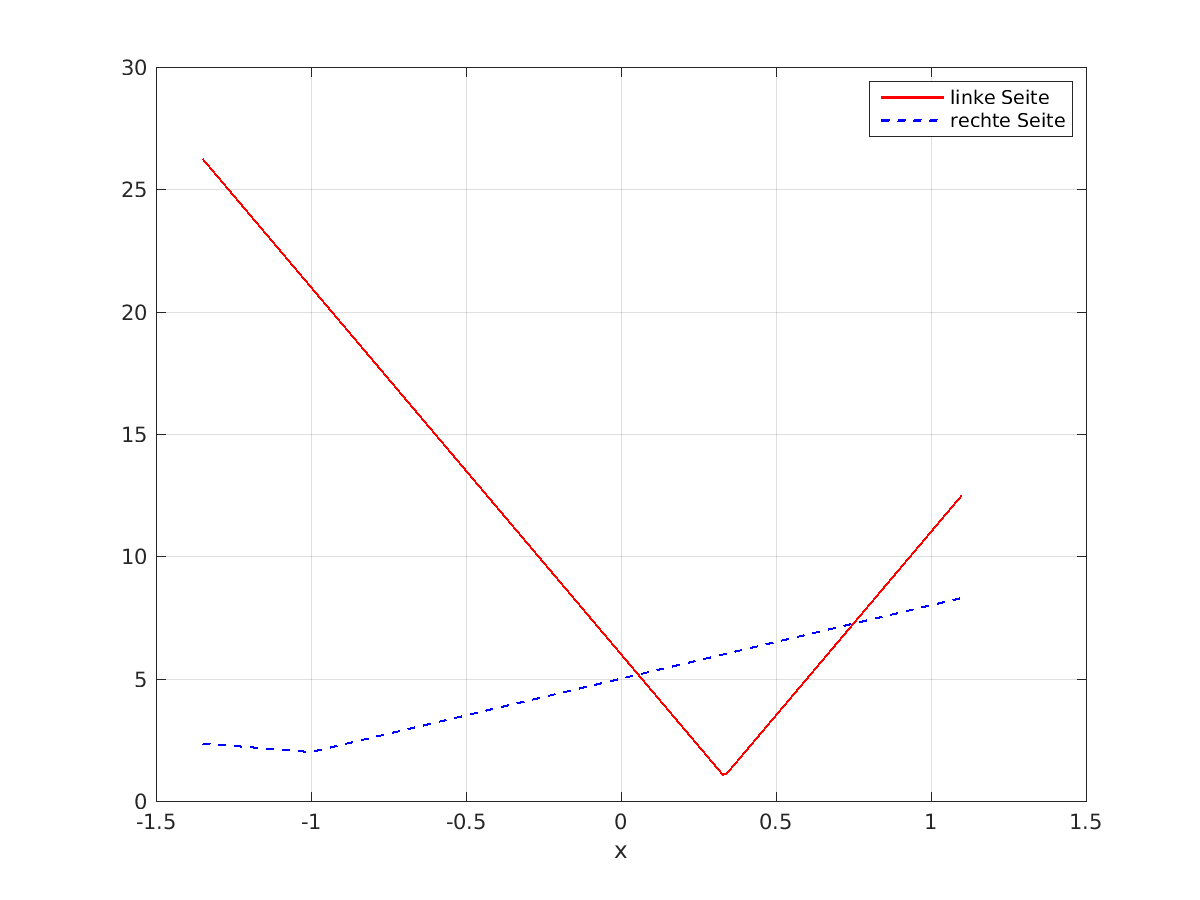
\includegraphics[width=0.8\linewidth]{Abb_zur_Ag_autogenerated_ineq_7.png} \end{center}
 
\else\relax\fi
 \end{MAufgabe}